\subsection{Texture Mapping}

Texture Mapping bezeichnet ein Shading-Verfahren, welches zweidimensionale Texturen auf ein dreidimensionales Objekt
abbildet. Um die flachen Texturen auf die Oberfläche des Meshs abbilden zu können, muss das Objekt 'UV-unwrapped' werden.
Durch diesen Vorgang wird jedem Punkt auf der Oberfläche des Meshs ein Punkt auf der Textur zugewiesen \parencite{Catmull1974} \parencite{Blinn1976}.
Ein sehr einfaches Beispiel zur Veranschaulichung ist dabei das Würfelnetz.
\textcolor{red}{>>GRAFIK VON WÜRFELNETZ/UV-UNWRAPPING<<}

Texture Mapping sorgt dafür die Objekte 'anzumalen'.
Reale Objekte haben oft sehr detaillierte Oberflächeneigenschaften und sind eigentlich niemals wirklich glatt.
Geometrische Unebenheiten und Feinheiten, wie Kratzer, Rillen und Schmutz lassen sich zwar mithilfe von
Texturen andeuten, jedoch bleibt die Oberfläche komplett glatt. Diese rauhen Oberflächen zu modellieren resultiert
aber in einer deutlich höheren Polygon-Anzahl, was die Performance in großen Szenen schnell negativ beeinflussen kann.
Daher wurden Mapping-Verfahren als Ergänzung entwickelt um die virtuelle Auflösung
solch komplexer Oberflächen kostengünstig zu erhöhen, ohne dabei die Komplexität der Geometrie zu verändern.
Dabei gibt es verschiedenste Shader, welche mithilfe weiterer, spezieller Texturen eine deutlich detailliertere
Oberfläche simulieren können.


% \subsubsection{Normal Mapping}
\subsubsection{Bump Mapping}

Eine Möglichkeit, mit der sich die Oberflächen mit mehr Details rendern lassen, ist das Rendering
mithilfe von sogenannten Bump Maps.
Hierbei werden mithilfe von Texturen, welche zusätzliche Informationen zu den Oberflächen enthalten,
Details generiert, welche den Eindruck einer realistischen Struktur der Oberfläche erzeugen. 
Dabei ist es nicht notwendig, dass die Geometrie an sich Informationen dazu beinhaltet \parencite{Blinn1978}.

Bump Maps sind Texturen, basierend auf Graustufen, bei denen die Helligkeit eines Pixels 
einen Höhenwert repräsentiert. Eine verbesserte Variante der Bump Maps sind die Normal Maps.
Hier werden die Richtungen der Normalen in jedem Pixel durch einen Vektor repräsentiert, 
welcher sich aus den RGB-Werten eines jeden Pixels ergibt. Daraus lassen sich Schattierungen simulieren,
welche kleine Unebenheiten (mit geringer Tiefe) wie Beulen oder Kratzer realistischer aussehen lassen. 
Dieser wird aus Lichtquellen, deren Einfallsrichtung und den Normalen aus der Textur berechnet. 
Somit wird auch bei geringer Polygonanzahl eine deutlich realistischer aussehende Oberfläche gerendert. 
\parencite{Cohen1998}.

Diese Texturen bieten einen sehr kostengünstigen
Ansatz um Tiefe zu simulieren, Shader basierend auf diesen Methoden sind dabei aber stark 
blickwinkelabhängig und sehen schnell unnatürlich verzerrt aus.
Von vorne betrachtet funktioniert die Illusion, je spitzer jedoch der Winkel zwischen Betrachter und
Oberfläche wird, desto auffälliger wird die Tatsache, dass die Silhouette des Objekts immer 
noch flach ist, da die Geometrie hierbei nicht verändert wird. 

\subsubsection{Displacement Mapping}
Mit Displacement Mapping werden dagegen tatsächlich mithilfe von Heightmaps die Positionen 
der Vertices entlang ihrer Normalen versetzt \parencite{Cook1984,Cook1987}. Dadurch kommt es nicht zu blickwinkelabhängigen Artefakten 
und die Illusion von Tiefe wird real. Objekte sehen aus einem flachen Winkel betrachtet nicht mehr 
glatt aus, sondern haben tatsächlich Struktur in ihrer Oberfläche. Damit dieser Effekt jedoch zustande kommt, 
muss das Mesh in einer gewissen Auflösung zur Verfügung stehen. Je nach Detailreichtum der Heightmap 
muss die Geometrie dabei in weitere Polygone unterteilt werden. Der Vorteil hierbei ist der hohe 
Grad an Realismus. Ein deutlicher Nachteil liegt dabei allerdings in der Performance. 
Ein weitgehender Einsatz von Displacement Mapping kann eine hohe Polygonanzahl schnell 
negativen Einfluss auf die Renderingzeiten nehmen.
\textcolor{red}{>>PERFORMANCEVERGLEICH MAPPINGVARIANTEN<<}

\subsubsection{Parallax Mapping}

Parallax Mapping (oder auch Offset (Bump-)Mapping) ist eine weiter Methode, um sich die Möglichkeiten von
Bump Mapping-Verfahren zu nutze zu machen. Anders als bei tatsächlicher Modifizierung der Vertices 
durch Displacement Maps werden hier nur die Texturkoordinaten abhängig vom Blickwinkel verschoben. \parencite{Kaneko2001, Welsh2004}
Durch Bewegung der Oberfläche oder des Betrachters entsteht somit ein realistischerer Eindruck 
von Tiefe in der Textur, welcher den des Displacement Mappings approximiert darstellt. 
Dabei ist Parallax Mapping allerdings immer noch deutlich effizienter als echtes Vertex-Displacement
und eignet sich daher eher für Echtzeitrenderings. Parallax Mapping alleine simuliert zwar den 
Parallax-Effekt, jedoch ist es hiermit nicht Möglich die Sillhoutte zu verändern und 
Selbstschattierung oder -verdeckung vorzutäuschen. 


\subsubsection{Parallax Occlusion Mapping}

Parallax Occlusion Mapping (POM) ist eine komplexere, verbesserte Variante des Parallax Mapping, basierend auf einem Per-Pixel Ray Tracing.

Das Ziel ist auch hier wieder das vorherige: Detaillierte Oberflächen ohne den Preis von Vertexdisplacements. 
Im Gegensatz zu klassischem Parallax Mapping berücksichtigt POM zusätzliche Eigenschaften wie Verdeckung und 
Selbstschattierung. 
Die Informationen aus der Heightmap werden hierbei jedoch für Berechnungen 
im Fragmentshader verwendet \parencite{Tatarchuk2006}. Dazu wird die Heightmap invertiert, denn anstatt
wie beim Displacement Mapping Details zu extrudieren wird bei POM in die Tiefe simuliert.  
Zunächst wird mittels Ray Casting vom Betrachter zur Mesh-Oberfläche ein Schnittpunkt ausfindig gemacht. 
Von dort wird mithilfe des ermittelten Punktes  

\begin{figure}[h]
    \centering
	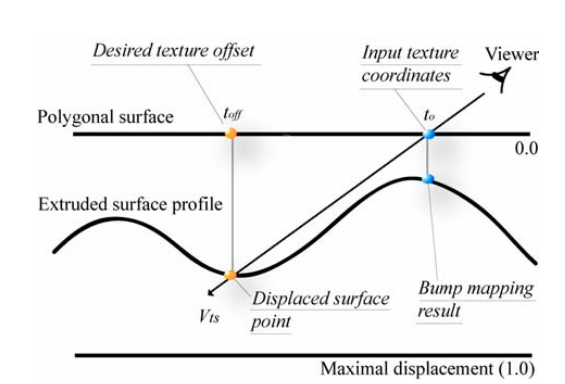
\includegraphics[width=0.8\textwidth]{Grafiken/POM.png}
	\begin{footnotesize}
		\caption{Parallax Occlusion Mapping}
	\end{footnotesize}
\end{figure}




% TODO:
% - Displacement Mapping kurz beschreiben -> Done
% - Parallax Mapping Nachteile -> Done
% - POM runterschreiben